% !TEX root = ../../I4PRJ, Grp3 - Dokumentation.tex
\section{Applikationslaget}
Dette afsnit beskriver implementeringen af applikationslaget. Implementeringen af applikationslaget best�r i, at implementere lagets modelklasser, presenterklasser og platform-specifikke user interface programmer. 

\subsection{Implementering af modelklasser}
Implementeringen af modelklasserne i applikationslaget beskrives i dette afsnit. Modelklasserne er implementeret i sproget C#, i Microsoft Visual Studio.

\subsubsection{Session.cs}
Session-klassen indeholder hovedsageligt properties, som kan overs�ttes direkte fra klassens design til kode. Da Session klassen er designet som en Singleton, beskrives implementeringen af dens constructor og statiske Session medlem i dette afsnit.

Listing~\ref{code:application_model_sharedsession} viser implementeringen af klassens statiske medlem. N�r SharedSession bliver brugt f�rste gang, laves en ny Session. I efterf�lgende brug returneres den statiske session fra backing variablen sharedSession.

\begin{lstlisting}[caption={SharedSession}\label={code:application_model_sharedsession}]
public static Session SharedSession => _sharedSession ?? (_sharedSession = new Session());
\end{lstlisting}

Listing~\ref{code:application_model_sessionconstructor} viser implementeringen af Session-klassens constructor. Constructor'en er gjordt privat, s�ledes at SharedSession beskrevet i listing~\ref{code:application_model_sharedsession}, er den eneste m�de man kan oprette en Session.

\begin{lstlisting}[caption={Session constructor}\label={code:application_model_sessionconstructor}]
private Session()
{
	SelectedPoolIndex = 0;
	Pools = new List<Tuple<string, bool>>();
}
\end{lstlisting}

\subsubsection{PoolLoader.cs}
PoolLoader-klassen indeholder en r�kke metoder til at hente data fra connection-serveren. Generelt opretter metoder en passende besked fra Smartpool.Connection.Model, sender den med en IClientMessenger, og parser evt. svaret der modtages fra serveren.

Listing~\ref{code:application_model_gcdfp} viser implementeringen af en af disse metoder. I metoden oprettes en GetPoolDataRequestMsg som instantieres med sessionsinformation fra Session-klassen. N�r svaret modtages, tr�kkes den relevante data ud af svarbeskeden, og laves om til en passende type.

\begin{lstlisting}[caption={GetCurrentDataFromPool(...)}\label={code:application_model_gcdfp}]
public List<Tuple<SensorTypes, double>> GetCurrentDataFromPool(IClientMessenger clientMessenger)
{
	var request = new GetPoolDataRequestMsg(_session.UserName, _session.TokenString, false, _session.SelectedPool.Item1);
	var response = (GetPoolDataResponseMsg) clientMessenger.SendMessage(request);
	return response.SensorList.Select(sensor => new Tuple<SensorTypes, double>(sensor.Item1, sensor.Item2.LastOrDefault())).ToList();
}
\end{lstlisting}

Klassen indeholder ogs� metoder der indl�ser data i den statiske Session-instans. Metoden i listing~\ref{code:application_model_reloadpools} er et eksempel p� dette. Metoden eftersp�rger pool-information fra serveren og gemmer den data der modtages i Session-instansen.

\begin{lstlisting}[caption={ReloadPools(...)}\label={code:application_model_reloadpools}]
public void ReloadPools(IClientMessenger clientMessenger)
{
	var poolRequest = new GetPoolDataRequestMsg(_session.UserName, _session.TokenString, true);
	var response = (GetPoolDataResponseMsg) clientMessenger.SendMessage(poolRequest);
	_session.Pools = response.AllPoolNamesListTuple;
}
\end{lstlisting}

\subsubsection{PoolValidator.cs}
PoolValidator-klassen indeholder de properties der blev defineret i klassens design, samt implementeringen af de tilh�rende funktioner. PoolValidator-klassens ansvar best�r i at tilbyde en m�de, at validere pool-oplysninger. Metoden i listing~\ref{code:application_model_pvisvalid} definere hvorn�r en pool anses som v�rende godkendt i systemet. Som det fremg�r af kodestykket, foretages en sammenligning af indholdet af klassens Name og SerialNumber properties.

\begin{lstlisting}[caption={IsValid()}\label={code:application_model_pvisvalid}]
public bool IsValid()
{
	if (Name.Length == 0) return false;
	if (SerialNumber.Length == 0) return false;
	return true;
}
\end{lstlisting}

Klassen indeholder ogs� funktionalitet, der tillader parsing af poolst�rrelse og volumen, fra string til double-repr�sentation. Listing~\ref{code:application_model_parsedvolume} implementerer denne funktionalitet. Metoden pr�ver f�rst at parse klassens volume property hvis den indeholder en string, hvis ikke, pr�ver fors�ger klassen at parse dimensions arrayet.

\begin{lstlisting}[caption={ParsedVolume()}\label={code:application_model_parsedvolume}]
private double ParsedVolume()
{
if (_volume != "")
	{
	_dimensions[0] = ""; _dimensions[1] = ""; _dimensions[2] = "";
	try
	{
		var volume = double.Parse(_volume);
		return volume > 0 ? volume : 0;
	}
	catch (Exception)
		return 0;
}
else
 {
	 _volume = "";
	try
		return double.Parse(_dimensions[0]) * double.Parse(_dimensions[1]) * double.Parse(_dimensions[2]);
	catch (Exception)
		return 0;
	}
 }
\end{lstlisting}

\subsubsection{UserValidator.cs}
UserValidator-klassen indeholder de properties der blev defineret i klassens design, samt implementeringen af de tilh�rende funktioner. Klassen kan validere brugeroplysninger, ved hj�lp af de metoder der ses implementeret i listing~\ref{code:application_model_uservalidator}.

\begin{lstlisting}[caption={UserValidator valideringsmetoder}\label={code:application_model_uservalidator}]
public bool PasswordIsValid => Passwords[0].Length >= MinimumCharacters && Passwords[0] == Passwords[1];
public bool IsValidForSignup => PasswordIsValid && Name.Length > 0 && Email.Length > 0;
public bool IsValidForLogin => Email.Length > 0 && Passwords[0].Length > 0;
\end{lstlisting}

Metoderne beskriver forskellige valideringsscenarier, og benytter klassens properties til at vurdere hvorvidt de indtastede oplysninger er tilstr�kkelige.

\subsection{Implementering af presenter-klasser}
Dette afsnit beskriver implementeringen af applikationslaget. Implementeringen af applikationslaget best�r i, at implementere lagets modelklasser, presenterklasser og platform-specifikke user interface programmer. 

\subsection{Implementering af view-klasser}}
Applikationslagets view-interfaces er blevet implementeret af klasser p� forskellige platforme, og beskrives derfor i deres egne afsnit. P� figur~\ref{fig:view_family} illustreres de f�rdigimplementerede brugergr�nseflader. 

\begin{figure}
	\centering
	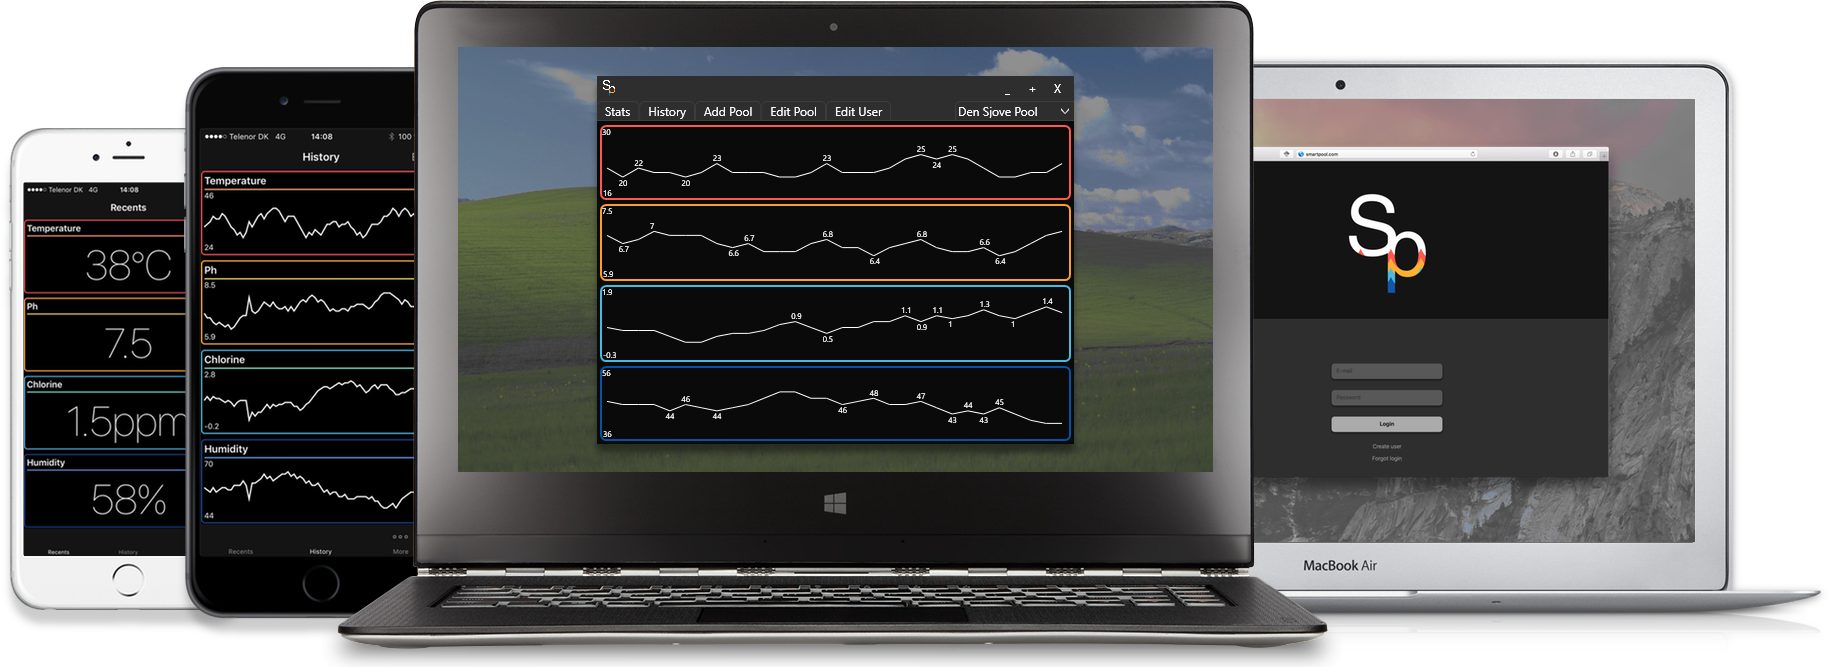
\includegraphics[width=1.0\linewidth]{figs/implementering/view_family}
	\caption{Brugergr�nsefladeimplementering p� hhv. iOS, Windows og Web}
	\label{fig:view_family}
\end{figure}